 %
%-----------------------------------------------------------
%% Computer Music Journal LaTeX template
%%
%% September  2009
%% Author: Cornelia Kreutzer, University of Limerick



%---Document preamble
%
\documentclass[letterpaper, 12pt]{article}


\usepackage{cmjStyle} %use CMJ style
\usepackage{natbib} %natbib package, necessary for customized cmj BibTeX style
\bibpunct{(}{)}{;}{a}{}{, } %adapt style of references in text
\doublespacing
\raggedright % use this to remove spacing and hyphenation oddities
\setlength{\parskip}{2ex}
\parindent 24pt
\urlstyle{same} % make url tags have the same font
\setcounter{secnumdepth}{-1} % remove section numbering
\usepackage{epstopdf}
\usepackage{amsmath,amssymb,amsbsy,bm,upgreek,nicefrac}
% \usepackage{todonotes}
\usepackage{microtype}

% Use the Figures subfolder for image files
\graphicspath{{./Figures/}}

%%%%%%%%%%%%%%%%%%% Begin MY PACKAGES %%%%%%%%%%%%%%%%%%%%%
% Uncomment only one of the ones below
\usepackage{anonymize} 		% Uncomment this line to publish
% \usepackage[blind]{anonymize}   %Uncomment this line for blind review

% \usepackage[firstpageonly=true, scale=1, colorspec=0.85]{draftwatermark} % draft watermark

\usepackage{enumitem}           % controls list spacing
\usepackage{longtable}
\usepackage{supertabular}
% \usepackage{pbox}
% \usepackage{caption}          % remove "Table x:" from Appendix
% \usepackage{url}              % hyperlinks 
% \usepackage{hyperref}         % to simplify the use of \href
% \usepackage{subfiles}         % add Appendixes as separate files
% \usepackage{pdfpages}         % include pdf pages for appendices

%=========== Tables ===========
\usepackage{multicol}           % span multiple columns in tables
\usepackage{multirow}           % span multiple rows in tables
\usepackage{tabularx}
\usepackage{tabulary}
\newcolumntype{L}[1]{>{\raggedright\let\newline\\\arraybackslash\hspace{0pt}}m{#1}}
\newcolumntype{C}[1]{>{\centering\let\newline\\\arraybackslash\hspace{0pt}}m{#1}}
\newcolumntype{R}[1]{>{\raggedleft\let\newline\\\arraybackslash\hspace{0pt}}m{#1}}

%%%%%%%%%%%%%%%%%%% End MY PACKAGES %%%%%%%%%%%%%%%%%%%%%


%% ----------------------------------------------------------------------------------------------------------------------------------------
%% CMJ page headers
%% For initial submission use \lhead{Anonymous}
%% On acceptance for publication, use real author surnames for \lhead modeled on the following examples
%%		One author:	\lhead{\small Keislar}
%%		Two authors:	\lhead{\small Keislar and Castine}
%%		Three authors:	\lhead{\small Keislar, Castine, and Rundall}
%%		Four or more:	\lhead{\small Keislar et al.}
%%
% \lhead{\small \anonymize{Sullivan, Wanderley and Guastavino}}
% \lhead{\small Sullivan, Wanderley and Guastavino}
\lhead{\small anonymous}


%% The package endfloat moves all floats (figures, tables...) to the end of the article, as required for the final version of a CMJ article.
%% Leave this package commented out for initial submission, but uncomment it and the following callout commands for the final version. 
% \usepackage{endfloat}
% \renewcommand{\figureplace}{%
%	\begin{center}
%		\textbf{<<TYPE: INSERT \figurename~\thepostfig\ ABOUT HERE.>>}
%	\end{center}}
% \renewcommand{\tableplace}{%
%	\begin{center}
%		\textbf{<<TYPE: INSERT \tablename~\theposttbl\ ABOUT HERE.>>}
%	\end{center}}

%---Document----------
\begin{document}


{\cmjTitle From Fiction to Function: Imagining New Instruments Through Design Workshops}
\vspace*{24pt}

% (In the initial submission, omit all the following author information to ensure anonymity during peer review.
% On final submission please make sure that the author address is a complete, functioning postal address.
% Post will be sent to that address.)

% Author: name
% {\cmjAuthor John Sullivan,\textsuperscript{*\dag} Marcelo M. Wanderley,\textsuperscript{*\dag} and Catherine Guastavino\textsuperscript{*\S}}	% List all authors here
{\cmjAuthor author names witheld for anonymity}	% List all authors here
							% e.g.:
							% {\cmjAuthor Doug Keislar, Peter Castine, and Jake Rundall}
 
% Author: address
\begin{cmjAuthorAddress}
    % \textsuperscript{*}Centre for Interdisciplinary Research in Music Media and Technology (CIRMMT) \\
    % \textsuperscript{\dag}Input Devices and Music Interaction Laboratory (IDMIL) \\
    % \textsuperscript{\S}Multimodal Interaction Laboratory (MIL) \\
	% McGill University\\
	% 527 Sherbrooke St. W. Suite A715 \\
    % Montreal, QC H3A1E3 Canada \\
	% \{john.sullivan2, marcelo.wanderley, catherine.guastavino\}@mcgill.ca
\end{cmjAuthorAddress}


\begin{abstract}
This paper introduces a set of workshops held with expert musicians to imagine novel musical instruments through design fiction. The workshops were based on the Magic Machine workshops developed by Kristina Andersen, in which participants crafted non-functional prototypes of instruments they would want to use in their own performance practice. Through in-situ activities and post-workshop thematic analysis, a set of design specifications were developed that can be applied to the design of new digital musical instruments intended for use in real-world artistic practice. In addition to generating tangible elements for design, the theories and methods utilized, based in human-computer interaction and human-centered design, are offered as a possible model for merging imaginative idea generation with functional design outputs. 

\end{abstract}

% \section{<<BEGIN ARTICLE>>}

% \section{Introduction}

Digital musical instrument (DMI) design is a broad and interdisciplinary field \citep{Miranda2006a}. Designers engage in the development of new instruments and novel approaches to musical performance (as well as composition and production) for a wide variety of reasons. Even where DMI design is fundamentally research-based, the means and the ends take a variety of forms, ranging from rigorous scientific experimentation to artistically motivated creative practice \citep{Gurevich2016}. Fittingly, the field, and more generally the broad domain of music technology in which it lies, contributes a wide range of outcomes both within and beyond specifically musical applications, such as the development of new technologies for interactive systems \citep{malloch2018generalized} and the advancement of knowledge and theories on technology-mediated artistic performance \citep{Tahlroglu2020}. 

With this work, we were interested to explore a novel method for the design of instruments expressly intended for real-world musical practice. Motivated by previous studies that examined key factors for user engagement \citep{OBrien2008} and long-term use of DMIs in performance \citep[\emph{reference removed for anonymity} (forthcoming), ][]{Wallis2013}, a workshop was held with expert musicians that led to a set of tangible design specifications for new performance DMIs. The workshop applied a user-driven approach to the early ideation stages of instrument development through the use of design fiction \citep{Blythe2014} and non-functional prototyping \citep{Pigrem2018} to inspire novel concepts for the new instruments. 

This article is structured as follows. First, we review motivations and methods for designing novel DMIs, focusing on existing theories and approaches drawn from human-computer interaction (HCI) and human-centered design (HCD). We then introduce the Design for Performance workshops and present results from thematic analysis of the sessions, which resulted in the set of design specifications. Finally, we discuss the potential of a design fiction approach to develop instruments that are viable for uptake and long-term use by expert musicians in real-world performance, and outline future work for robust evaluation of the methods explored.

\section{Background}
\label{sec:background}

An important aspect of the progression from acoustic to electronic and digital instruments has been the decoupling of the user input from sound production, leaving the designer free to choose any type of input control and mapping paradigm to control sound production. This freedom may be welcome, as evidenced by the quantity, complexity and diversity of new DMIs that have been developed over the last few decades. However this may also present a challenge for designers, when ``any bodily gesture can be mapped to any sound and there is no natural paradigm at play that we can relate to'' \citep*[p. 34]{Magnusson2019}. While the issue of mapping is a deep area of research and scholarship in its own right (see \citet{os-mapping-2002} and \citet{cmj-mapping-2014} for in-depth reports), here we focus on two more basic inquiries: First, if few technical and conceptual limitations exist, what motivates the design of new DMIs? And second, what methods can be applied to the development of novel DMIs that will make them appealing for use in artistic practice? 

\subsection{Diverse motivations for designing new instruments}
\label{sec:diverse-motivations-for-designing-new-instruments}

There are a wide range of factors that motivate the design of DMIs. In research settings, it may be useful to design DMIs that are specific to a particular experimental context \citep{Marquez-borbon2011}. A survey by \citet{Morreale2017} of DMI designers presenting instruments at the International Conference on New Interfaces for Musical Expression (NIME) found this to be a common approach: out of the 97 instruments included in the study, 38 (39\%) were reported to have been designed as research probes. In these circumstances, the instruments' actual use in real-world performance may be of secondary importance to more immediate research objectives. When considering performance with new instruments in more widespread and particularly non-research contexts, social, cultural, and economic factors come into play, in particular market and consumer-driven behaviors that influence trends, popularity, and visibility of commercial, off-the-shelf instruments \citep{Theberge1997}. The diversity of design approaches and objectives (in particular between commercial and research-based designs) has been highlighted by \citet{mcpherson2019musical} in a comparison of instruments emerging from different domains including NIME, HCI, and crowdfunding campaigns. 

\citet{Emerson2018} focus specifically on the design of DMIs expressly intended for artistic practice, identifying four primary categories of motivation: facilitating greater embodiment in performance, improving audience experience, developing new sounds, and building responsive systems for improvisation. They also highlight different motivations based on the context of participants' practices: those more active in academic settings exhibit more interest new sounds and responsive systems for improvisation, while others who perform in club settings are motivated to improve embodiment and audience experience. While not discussed by the authors, this might also be a correlation to the type of music they perform with their instruments. 

\subsection{DMI design and HCI}
\label{sec:dmi-design-and-hci}

The diverse motivations for designing new instruments are also reflected in various design approaches and methodologies used. Part of the discourse on DMI design comes from the field of HCI, which over time has evolved from quantitative and rigid strategies \citep{Bodker2015} to paradigms that are better suited to accommodate idiosyncratic approaches that are frequently found in music interaction contexts \citep{Wanderley2002}. Second wave HCI emerged to include perspectives on technology within social, cultural and organizational contexts \citep{kaptelinin2003} with an emphasis on user-centered, qualitative methods theoretically grounded in situated action, distributed cognition, and activity theory \citep{Bodker2006}. The third wave has continued to expand the purview of HCI to accommodate the ubiquitous nature of technology, prioritizing experiences, meaning-making, and emergent use \citep{Bodker2015}. This third paradigm is phenomenologically situated with a focus on embodied interaction to embrace multiple interpretations and yield rich understandings \citep{Harrison2007}, supported by ethnographic and practice-based research approaches \citep{Bodker2015}.

\subsubsection{User-centered, human-centered and participatory design}
\label{sec:user-centered-design}

User-centered design (UCD) requires the designer to ``ask what the goals and needs of the users are, what tools they need, what kinds of tasks they wish to perform, and what methods they prefer to use'' \citep[\citeauthor{Norman1988} \citeyear{Norman1988}, as cited in][p. 44]{El-shimy2014}. Human-centered design has emerged as a subtle but important variation \citep{Norman2013}, allowing for a broader consideration of people with regards to design, instead of ``a narrower focus on peoples' roles as users'' \citep[p. 45]{Steen2011}. This corresponds with trends in HCI: ``Instead of focusing on how specific tools can be designed to help users accomplish specific tasks, the human-centered perspective encourages developers to strive for a better understanding of how people live in the world, and to design systems accordingly'' \citep[p. 45]{El-shimy2014}. In DMI design, the concept of ``musician-as-user'' has been challenged more recently by \citet{Rodger2020}, who argue that there is no prototypical `user' for a given instrument, and characterizing musical activity is highly dependent on the context in which it occurs.

Participatory design (PD) is an HCD approach that became well-established with second-wave HCI \citep{Bodker2015} and has continued to be relevant in third-wave HCI as well \citep{Muller2012}. It is predicated on the full participation of end-users through all stages of the design process \citep{Steen2011}, and is primarily concerned with the \emph{tacit knowledge} of the involved participants which, according to \citet{Spinuzzi2005}, is hard to formalize and had been missing from early HCI. In DMI research, PD methods have been applied in the design and evaluation of Theremin-based controllers \citep{Geiger2008}, audio-haptic interfaces for the visually impaired \citep{Metatla2016}, and more generally to investigate music interaction design based on conceptual metaphor theory \citep{wilkie2013towards} and digital musical interaction ecologies \citep{Fyans:2012}.

It is important to note that PD is rooted in social activism and was originally envisioned as a way ``to rebalance power and agency among managers and workers'' \citep[p. 1]{Bannon2018}. Some current PD practices have been critiqued as merely UCD by a different name, lacking the original political and activist contexts \citep{Bannon2018}. Our own work presented here uses methods that fall under the PD umbrella but without any specific political motivation; therefore we identify our approach as HCD in deference to these objections.

\subsubsection{Design frameworks and novel approaches to idea generation}
\label{sec:design-frameworks}

Many different frameworks have been developed for the design and evaluation of new DMIs. Examples include models based on categories of musical interaction \citep{Bongers2000a}; structural components of DMIs \citep{Wanderley2004}; diverse needs of different performers \citep{Jorda2004, Jorda2004b}; interdisciplinary approaches combining music performance, HCI, and digital technology \citep{Overholt2009}; and user experience tracking \citep{fmorreale:2014}. Evaluation frameworks include include those based on user tasks \citep{Wanderley2002}; the roles of various stakeholders \citep{OModhrain2011a}; and formal HCI techniques for assessing functionality, usability, and user experience \citep{Young2015a}.

While high level design frameworks may be helpful in formulating a conceptual approach, they are generally not oriented towards specific design tools and methods or their use in artistic contexts. For our own work, we wish to develop effective strategies for developing new instruments that will be appealing for musicians to incorporate into their real-world creative practice. In particular, we look at two user-driven approaches to generating ideas for new designs: a physical DMI prototyping toolkit and a design workshop methodology. 

\subsubsection{Probatio}
\label{sec:probatio}

Probatio is a system developed by \citet{Calegario2017} that is comprised of a set of physical modules and accompanying methodology for exploring ideas and developing proof-of-concept DMI prototypes. It is meant to address a few important issues that arise in DMI design: for one, it provides functional constraints to limit the endless possibilities and increased complexity that arises from the separated user input and sound production components of DMIs, which can lead to ``creative paralysis'' \citep{Magnusson2010}. For another, it can help speed up and eliminate bottlenecks for iterative design, facilitating rapid design and evaluation cycles. The Probatio hardware consists of several control blocks, each featuring a different type of input control (ie., buttons, slider, crank, etc.), and different bases and structural supports that can accommodate variable configurations of the control blocks. The hardware is engineered so that the blocks attach magnetically and electrical connections are made automatically. Control signals are then mapped to sound synthesis software, making the prototype instantly playable as soon as one or more blocks are connected. An example Probatio prototype is shown in Figure \ref{fig:probatio-assembly}.

\begin{figure}[htbp]
    \begin{minipage}{0.49\textwidth}
        \centering
        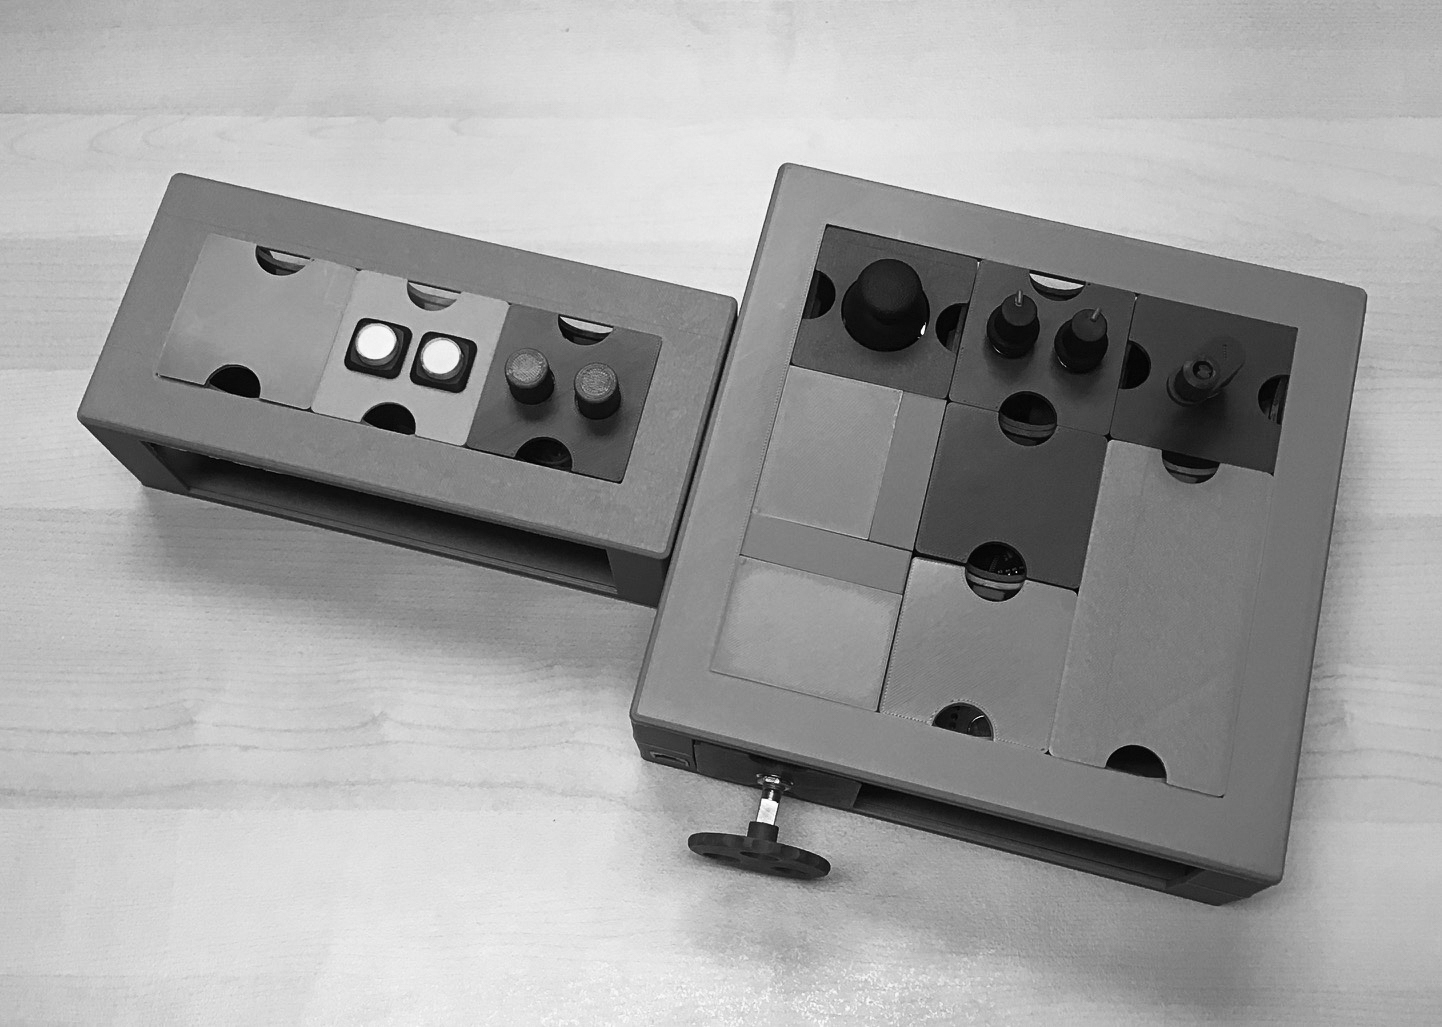
\includegraphics[width=1\textwidth]{probatio_assembly.jpg}
        \caption{Probatio prototype constructed from base, structural support and multiple control modules \citep{Calegario2020}.}
        \label{fig:probatio-assembly}
    \end{minipage}\hfill
    \begin{minipage}{0.49\textwidth}
        \centering
        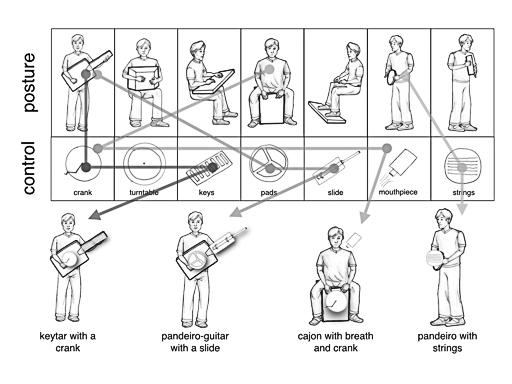
\includegraphics[width=1\textwidth]{probatio_chart.jpg}
        \caption{Morphological chart suggesting new prototypes by combining features of existing instruments \citep{Calegario2020}.}
        \label{fig:probatio-chart}
    \end{minipage}
\end{figure}

The methods that guide the use of the Probatio toolkit are based on Calegario's concept of \emph{instrumental inheritance} in which aspects of existing instruments such as physical structures, playing techniques, and specific types of input controls can be explored in different combinations and configurations, yielding entirely new instruments. A morphological chart \citep{Cross2000}, shown in Figure \ref{fig:probatio-chart}, assists the designer in this process, presenting different postures and controls that can be constructed with the Probatio hardware.

\subsubsection{Magic machines and design fiction}

Another compelling approach to idea generation and prototyping for DMI design comes with ``Magic Machine'' workshops developed by \citet{Andersen2017}. The workshops ``make use of the notion of technology as a `magical unknown' as the starting point for a range of workshop techniques that begin with material exploration'' \citep[p. 4971]{Blythe2016}. In them, participants are prompted to make non-functional low-fi prototypes out of generic crafting materials like cardboard, wood, string, and glue. Once finished, they present their creations, demonstrating their use in imagined scenarios.

The Magic Machine workshops have some basis in design fiction, where concepts and problems can be explored through the development of imaginary scenarios and ``fantasy prototypes'' \citep{Sterling2009}. Importantly, the artifacts that are generated (the non-functional prototypes) are not overly meaningful in and of themselves, and the ultimate aim is not solve any given problem. Rather, the processes of creating and engaging with the ``magical unknown'' serves ``to give temporary body to concerns and questions [and] to consider the potential reality of a world in which such a thing might exist'' \citep[p. 4971]{Blythe2016}. Andersen has run the workshops is a variety of of contexts for both adults and children, including workshops for the design of new (imagined) musical instruments. The workshop has been used by other DMI researchers as well, including a study by \citet{Lepri2019} that explored diverse values and priorities of different music cultures, backgrounds, and contexts.

\subsubsection{Towards design for performance}
\label{towards-design-for-performance}

The Probatio toolkit and Magic Machine workshops present dynamic methods for early ideation stages of DMI design that we are interested in applying to our own work. The workshops offer a creative approach for generating ideas free from technological or practical constraints, while Probatio provides a clearly defined set of tools to quickly construct and evaluate prototypes. 

\section{The Design for Performance workshop}
\label{sec:design-for-performance-workshop}

The Design for Performance workshop was developed to involve expert musicians in the early stage ideation of new instruments, and draws from a variety of general methods from HCD and PD that have been mentioned so far: design workshops, non-functional and low-fidelity prototyping, and design fiction. The structure is based on Andersen's Magic Machine workshops but is revised to direct the outcomes towards the generation of design specifications that could be applied to the development of new performance-ready DMIs. 

The context of the Design for Performance workshops marks an important shift from Andersen's Magic Machine workshops, which are specifically oriented towards building diverse design knowledge and complex understandings ``about technology, rather than of technology'' \citep[p. 1]{Andersen2019}. Our approach seeks to find a middle ground between theoretical knowledge and tangible design, connecting the diversity and creative freedom fostered by the Magic Machine activities with a holistic design ecology from ideation to finished product. In this way, the Design for Performance workshop is envisioned as a design tool that can elicit preliminary ideas from a group of expert practitioners and translate them into tangible elements that designers can work with. This may be especially valuable in the DMI design space, where idiosyncratic approaches and highly personalized designs are common, and widespread adoption of new DMIs is limited.

\subsection{Pilot}
\label{sec:pilot}

A pilot test was carried out to run the full workshop from start to finish. Six master's students who were enrolled in a graduate seminar about musical interface design participated. The session was facilitated by the first author who was assisted by another master's student. The session was observed by two colleagues of the facilitator (a music technology Ph.D. student and visiting professor). After the session an informal discussion was held with the participants and observers to get feedback and take suggestions for any improvements that could be made. All generally agreed on the activities and format, while details for minor changes were noted and incorporated into the final structure.  

\subsection{Participant recruitment}
\label{sec:participant-criteria-and-selection}

As the workshop was focused on the design of DMIs for use in live performance and intended to be held with expert musicians, we identified three main criteria for prospective participants: 1) they should use, or at least be familiar with, DMIs; 2) they should maintain an active performance practice (performing publicly at least five times per year); 3) their performance practice should be related to styles in which DMIs are typically used, such as electroacoustic and experimental styles.

A call for participation was circulated through local academic and performance community mailing lists that were likely to reach individuals matching our criteria. Interested parties were invited to complete an online prescreening questionnaire. Recruitment lasted for two weeks and 25 responses were received. 15 individuals met the criteria and were invited to participate, of which ten accepted. To accommodate schedules, the workshop was divided into two sessions, with three participants in session A and seven in the session B. 

The workshop activities and procedures were reviewed and approved by the Research Ethics Board Office of {\emph{university name removed for anonymity}}
% McGill University
and all participants read and signed a form of informed consent before beginning. 

It should be noted that three of the participants were known by the authors. In particular, P09 is an instrumental performer and regular collaborator with the first author. Given the limited size of the local DMI community, we determined that it should not disqualify them from participation if they met the defining criteria.

\subsection{Workshop activities}
\label{sec:workshop-activities}

A schedule for the workshop had been developed based on Andersen's recommendations to run the workshop at a quick pace and keep a tight timeline. This was found to be an effective strategy to alleviate any potential anxieties or fears of failure that participants could experience during the creative and open-ended design activities \citep{Andersen2017}. The sessions were held on consecutive days in a spacious and well lit conference room at 
{\emph{location removed for anonymity}}.
% the Centre for Interdisciplinary Research in Music Media and Technology (CIRMMT) at McGill University. 
Tables were arranged together so that participants sat around the outside facing each other. A variety of crafting materials was arranged on a separate table and covered with a cloth when the participants arrived. A videocamera was set up to record the sessions.

The first author acted as the facilitator and was aided by the same assistant from the pilot session. Each session began with a welcome and introduction by the facilitator, then participants were asked to briefly introduced themselves and give a short summary of their musical practice and experience with DMIs. 

\subsubsection{Activity 1: Prompt}
\label{sec:activity-1-prompt}

The workshop activities began with a prompt. Participants were asked to think of the music that currently make or would like to make, and then instructed to ``draw the music'' on an index card in front of them with a permanent marker. They were given two minutes to complete the activity, after which the workshop moved directly on to the next activity.
% In the Magic Machine version the drawing is made on the participant's own hand, however this was opposed in the pilot so the drawing was moved to an index card instead.
% Prompts and icebreakers are commonly used in workshop settings to initiate a session, putting the participants at ease and orienting them to the problem at hand. 

Andersen stipulates two important functions that this activity serves. First, it provides the specific context for the workshop focus. 
% In this case, the focus is on designing new musical instruments, therefore 
Drawing the participants' attention to making music in novel and unexpected ways (as suggested by the inherent absurdity of \emph{drawing} music) oriented focus to thinking creatively about instruments and performance. Second, the short activity serves as a preliminary task to complete, ``an initial goal\ldots that tests competence and establishes confidence, acting as an on-ramp to an experience'' \citep[p. 5]{Andersen2019}. This eases the transition into to the more substantial design activity that follows, as one creative task has already been completed. 

\subsubsection{Activity 2: Crafting non-functional prototypes}
\label{sec:activity-2-crafting-non-functional-prototypes}

In this main activity of the workshop, ``the content of the prompt must be translated into an imagination of the device that produces it'' \citep[p. 5]{Andersen2019}. The use of rudimentary crafting materials moves the focus away from producing high resolution or even technically feasible designs. Instead, the participants are asked to envision and craft a purely fictional instrument that they would want to use, and the materials (and especially their unsuitability for functional instrument design) allow the participant to operate freely and instinctively without concern for implementation or technical constraints.

Participants were directed to construct an instrument with which they could play the music they had drawn, using the basic crafting materials provided that included items such as poster board, colored index cards, sticks, disposable plates and cups, tape, markers, string, and wire. The facilitator emphasized that they were to build non-functional prototypes and that they should neither utilize materials for their acoustic properties nor be concerned with technical feasibility. The groups were given 30 minutes to complete the activity. Figure \ref{fig:instrument-building} shows the groups building their prototypes.

\begin{figure}[t]
    \centering
    \begin{subfigure}[]{1\textwidth}
        \centering
        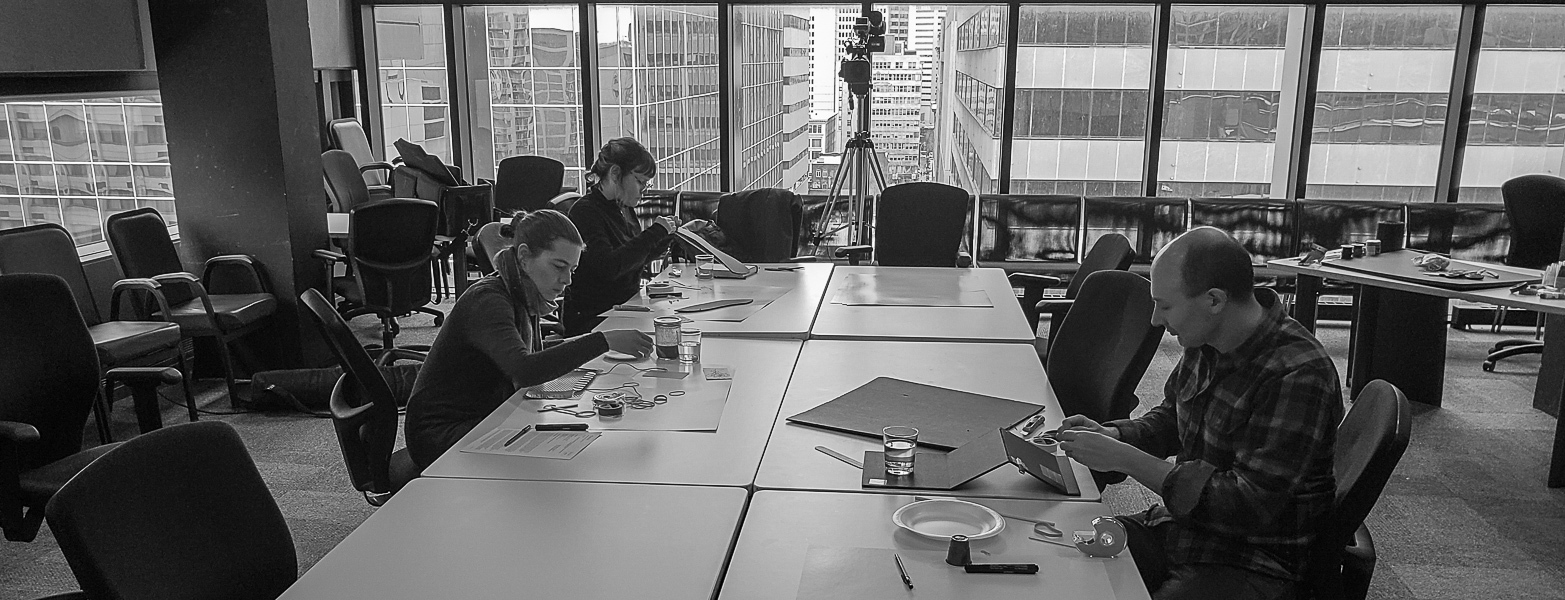
\includegraphics[width=1\textwidth]{dfp_nfp_A.jpg}
        \caption{Session A}
        \label{fig:keybox-cad}
    \end{subfigure}
    \par\bigskip
    \begin{subfigure}[]{0.59\textwidth}
        \centering
        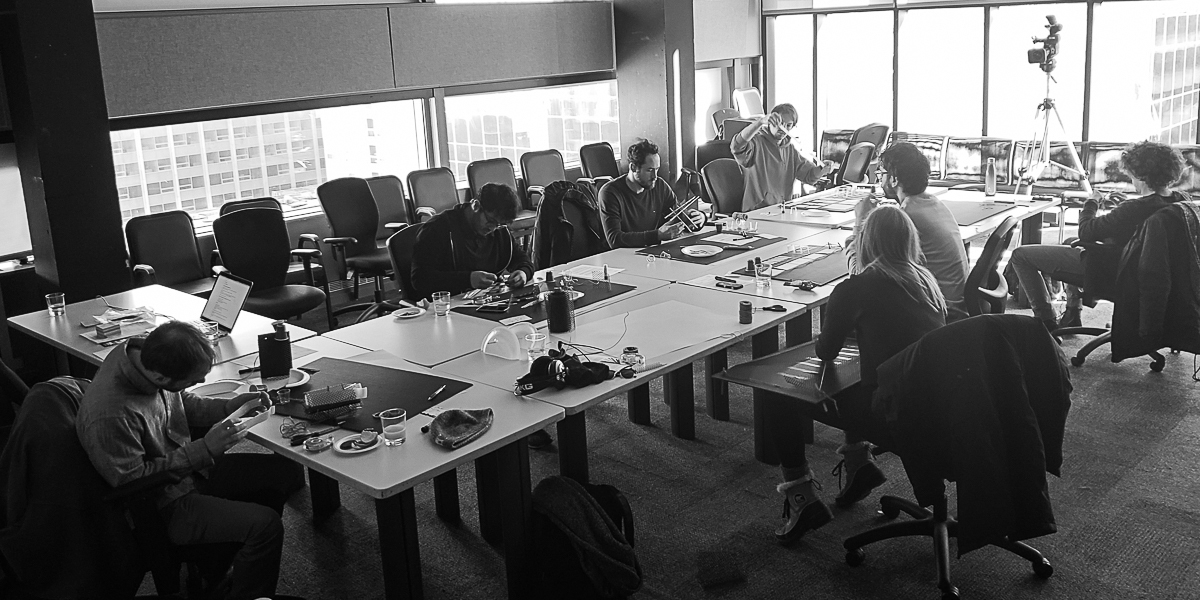
\includegraphics[width=1\textwidth]{dfp_nfp_B.jpg}
        \caption{Session B}
        \label{fig:stringbox-cad}
    \end{subfigure}
    \begin{subfigure}[]{0.4\textwidth}
        \centering
        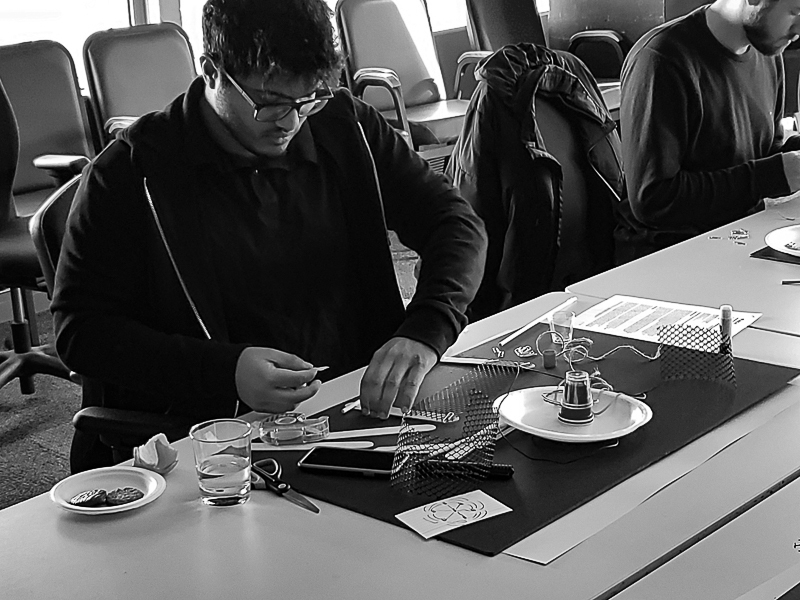
\includegraphics[width=1\textwidth]{dfp_nfp_B_P4.jpg}
        \caption{Participant P04 in Session B}
        \label{fig:tapbox-cad}
    \end{subfigure}
    \caption{Participants crafting non-functional instrument prototypes in Activity 2.}
    \label{fig:instrument-building}
\end{figure}

To assist the participants in developing their ideas into tangible designs, we introduced an informal list of eight considerations to refer to while building their instruments, which were written on a large whiteboard. The considerations are divided into two categories: (1) high-level operational qualities and general characteristics that could describe the instrument's intended use (\emph{functionality}, \emph{playability}, \emph{musicality}, \emph{performance context}), and (2) low-level essential features and fundamental components of the design (\emph{physical form and ergonomics}, \emph{interaction methods}, \emph{sound production}, \emph{feedback}). While some of the considerations can be classified as functional and non-functional requirements (as defined by requirements engineering \citep{Glinz2007} and commonly employed in systems design), it is important to point out that these elements were empirically chosen based on our own prior knowledge and experience in DMI design, and left open-ended to provide helpful points of reference through the activity. 

\subsubsection{Activity 3: Presentations and key element identification}
\label{sec:activity-3-presentations}

Following the construction, each participant gave a three minute presentation of their instrument. Participants were encouraged to explain the links between the music on their index cards and the instruments, which helped to orient the presentations on the imagined outcomes rather than the technical details of the fabricated designs. A two minute group discussion followed each presentation. 

While the participants described their instruments the facilitator noted key elements of their designs, such as essential features, attributes, characteristics that could help to define the instrument. These elements were written on sticky notes and posted to the whiteboard, clustered around the eight considerations that had been given in the previous activity. The presenter and other participants were encouraged to suggest elements to add the the board as well.

\subsubsection{Activity 4: Dot-voting}
\label{sec:activity-4-dot-voting}

The key element identification was intended to allow the group collectively to consider aspects of the designs that would be appealing to incorporate into a fully functional instrument. When the presentations were finished, participants were then asked to vote for the elements that they most strongly favored by placing colored stickers (dot votes) next to the items they wished to vote for (as shown in Figure \ref{fig:dot-voting}). Each participant was allotted 10 votes, based on the average number of participants per session and recommendations by \citet{Gray2010} and \citet{Gibbons2019}. 

\begin{figure}[htbp]
    \begin{minipage}{0.49\textwidth}
        \centering
        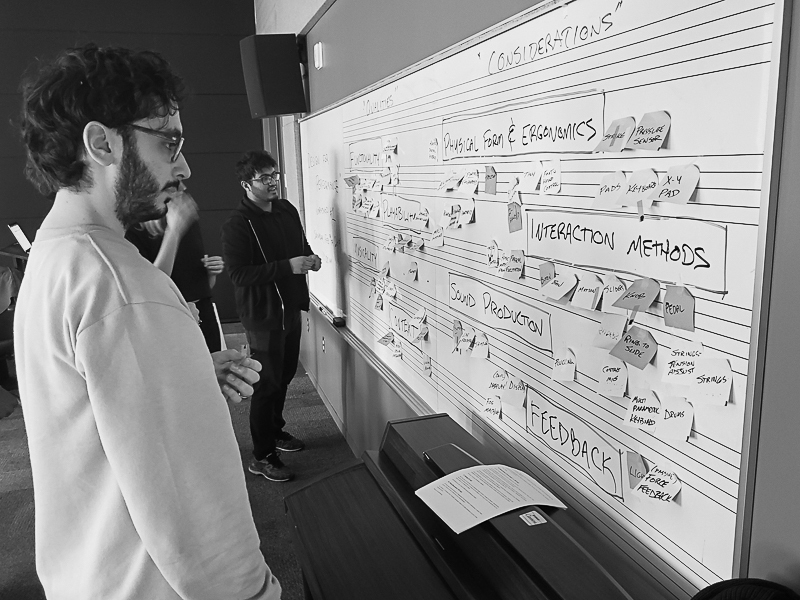
\includegraphics[width=1\textwidth]{dfp_dot_voting_B.jpg}
        \caption[Design for Performance workshop: Activity 4 - Dot voting]{Session B participants dot voting for essential design elements in Activity 4.}
        \label{fig:dot-voting}
    \end{minipage}\hfill
    \begin{minipage}{0.49\textwidth}
        \centering
        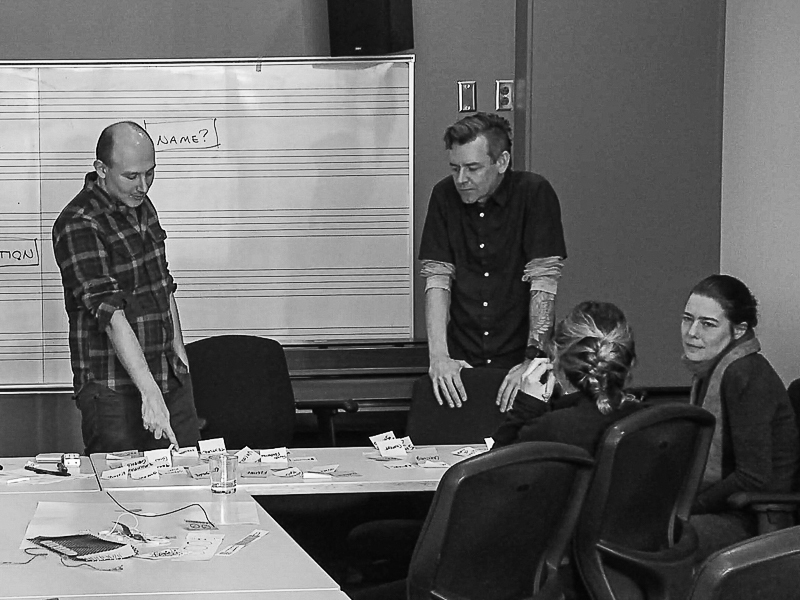
\includegraphics[width=1\textwidth]{dfp_discussion_A.jpg}
        \caption[Design for Performance workshop: Activity 5 - Discussion]{Session A participants conclude the workshop with a group discussion in Activity 5.}
        \label{fig:discussion}
    \end{minipage}
\end{figure}

\subsubsection{Activity 5: Group discussion}
\label{sec:activity-5-group-discussion}

The workshop concluded with an open discussion (shown in Figure \ref{fig:discussion}) with the facilitator and participants about the identified key elements and prospects for utilizing them in the development of new DMIs that they would want to use in their own practice. The facilitator also provided information about future steps for the project including the eventual design of functional instrument prototypes based on the workshop outcomes. The workshop length for session A with three participants was 90 minutes. Session B, with seven participants, was completed in just under two hours. 

\section{Results}
\label{sec:results}

Workshop results are reported in two parts. First we present the direct outcomes of the workshop activities, then we present results from thematic analysis of the video recorded workshop sessions. 

\subsection{Participant profiles and output}
\label{sec:participant-profiles-and-output}

In addition to the basic background information collected in the prescreening questionnaire, the self introductions at the beginning of the workshop provided additional insights about the participants' own musical and DMI practices. Profiles of the ten participants are shown in Appendix 1.

During the self introductions, participants were also asked if they had previous experience with designing digital musical instruments. While this was not a criteria for participation, six of the participants reported at least some previous experience, including P04 and P05 who come from engineering backgrounds and have significant technical knowledge and experience in this area. This is consistent with DMI literature that highlights the overlap between DMI design and practice (see \citet{Magnusson2008, Morreale2017, Morreale2018} for example). While not a specific focus for this study, we can envision a future workshop variant that investigates the differences between designers and non-designers explicitly.

\subsubsection{Design outputs}
\label{sec:design-outputs}

During the workshop each participant produced two physical design artifacts: their ``draw the music'' index card (as described in the presentations) and the instrument prototypes. The outputs are listed in Appendix 2, with instruments categorized according to \citeauthor{Miranda2006a}'s classification of gestural controllers (\citeyear{Miranda2006a}): \emph{augmented}, \emph{instrument-like}, \emph{instrument-inspired}, and \emph{alternate}. As the drawing of the cards was done as a prompt for the main activity, they are not examined here. 

\begin{figure}[t]
    \centering
    \begin{subfigure}{0.49\textwidth}
        \centering
        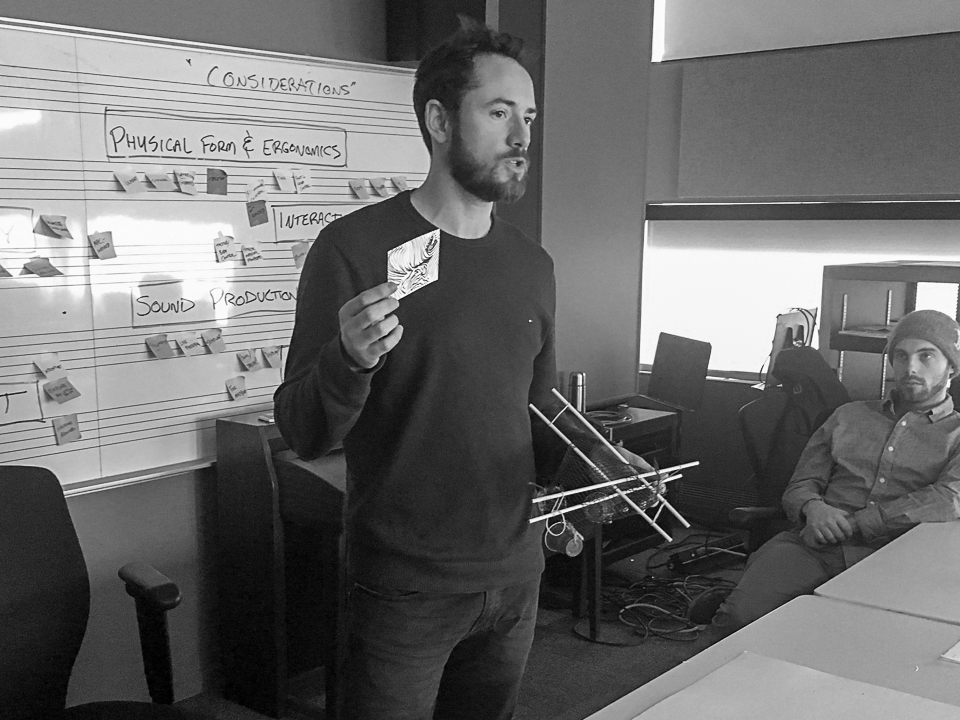
\includegraphics[width=1\textwidth]{P05.jpg}
        \caption{P05}
        \label{fig:presentations_P05}
    \end{subfigure}
    \begin{subfigure}{0.49\textwidth}
        \centering
        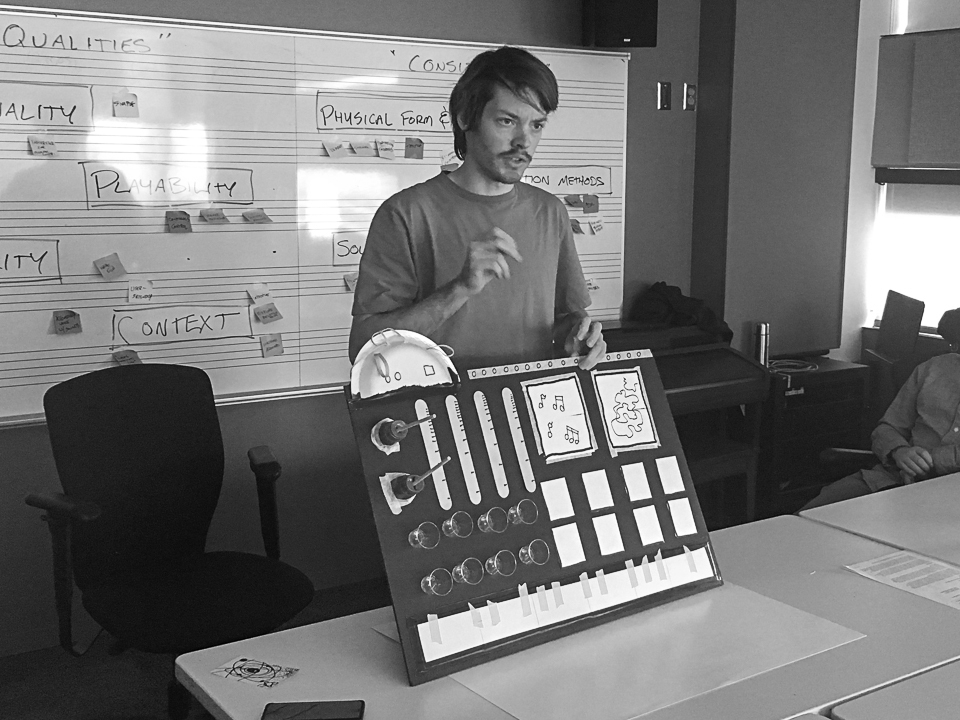
\includegraphics[width=1\textwidth]{P06.jpg}
        \caption{P06}
        \label{fig:presentations_P06}
    \end{subfigure}
    \begin{subfigure}{0.49\textwidth}
        \centering
        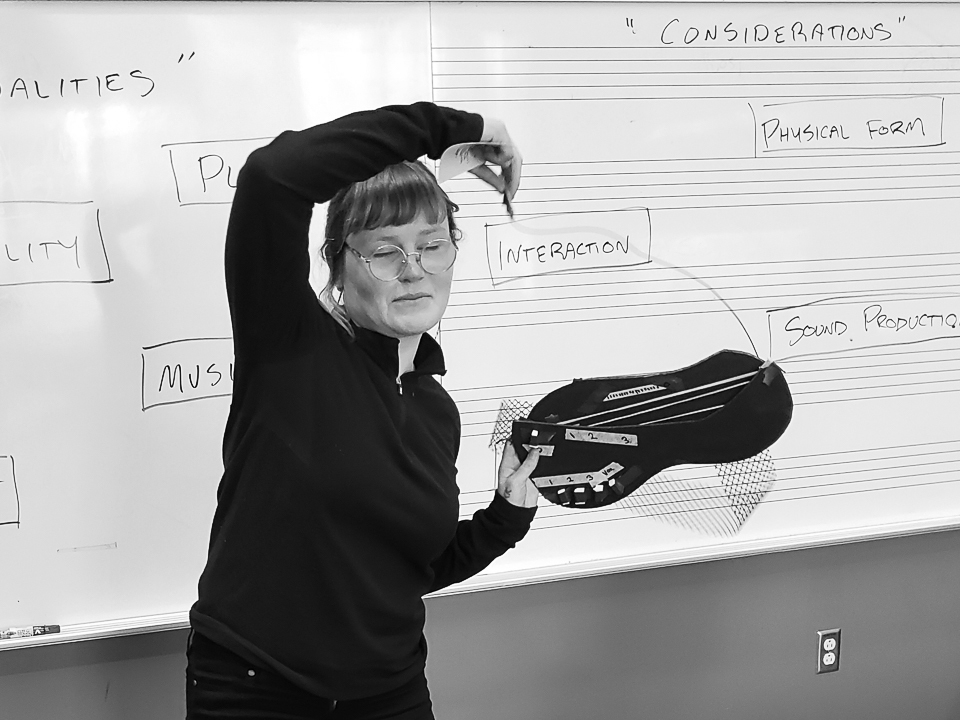
\includegraphics[width=1\textwidth]{P02.jpg}
        \caption{P02}
        \label{fig:presentations_P02}
    \end{subfigure}
    \begin{subfigure}{0.49\textwidth}
        \centering
        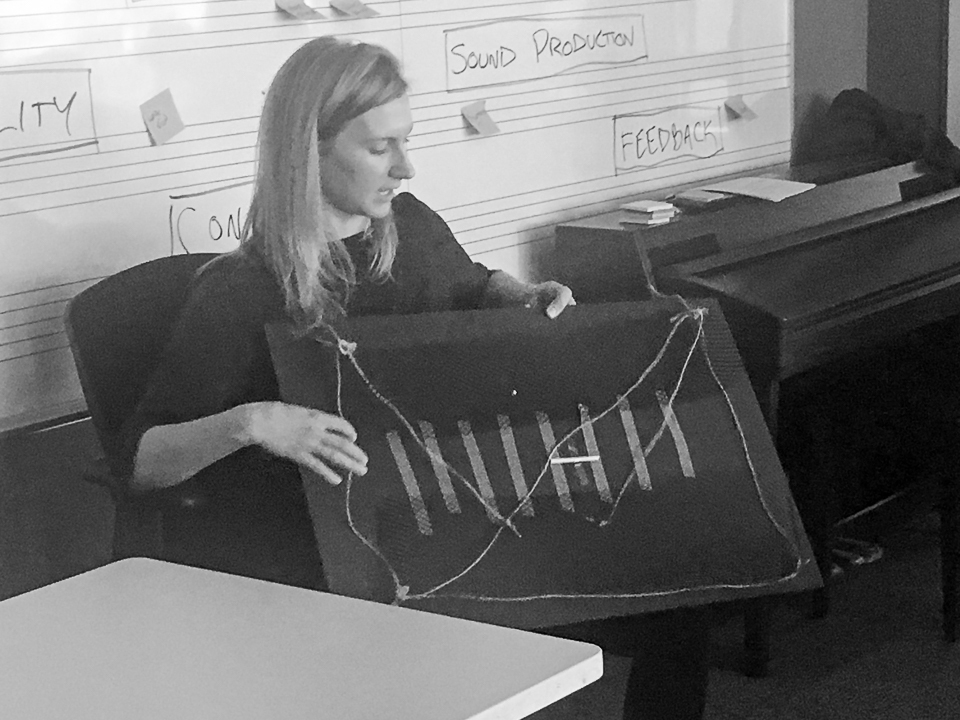
\includegraphics[width=1\textwidth]{P09.jpg}
        \caption{P09}
        \label{fig:presentations_P09}
    \end{subfigure}
    \caption{Participants present their instrument prototypes in Activity 3.}
    \label{fig:presentations}
\end{figure}

Half of the instruments can be classified as alternate instruments, and bear little or no resemblance to existing instruments. While each was entirely unique, the various forms show the strong influence the materials played on the resulting designs, with each instrument prioritizing physical shapes and textures as the focus of the design. For example, P05 created a resonant physical structure built of many different types of materials (Figure \ref{fig:presentations_P05}). The structure would be excited by touching, tapping, rubbing or plucking different elements, which would generate audio signals to drive multiple different sound processes.

Four of the remaining five instruments can be identified as either instrument-like or instrument-inspired, taking various elements from existing instruments and repurposing them in different ways. A noticeable trend among this group was to combine the functionalities of several instruments into a single instrument, either to be able to play multiple parts simultaneously like P06's multifunction performance workstation (Figure \ref{fig:presentations_P06}) or to mix them together in creative ways like P02's instrument that would mix and cross-modulate vocals and guitar (Figure \ref{fig:presentations_P02}). 

There was one augmented instrument designed by P09 (Figure \ref{fig:presentations_P09}). This participant is an expert instrumentalist with an advanced degree in performance on her instrument, the concert harp. She has been performing electroacoustic music using harp and various external controllers including custom interfaces designed by the first author 
(\emph{reference removed for anonymity} 2018)
% \citep{Sullivan2018}
and was clear in her needs and priorities as a performer, which was reflected in the pragmatic approach and practical utility of her design. 

\subsection{Key elements, dot voting and discussion}

As described previously, during presentations key elements of the participants' prototypes were identified and posted to the whiteboard. Afterwards the participants were asked to dot vote for the elements that they would most want to be incorporated into a new instrument design. In the planning of the workshop, we imagined these activities could serve two purposes. First, they could provide direct, quantifiable data that could be applied towards the eventual development of design specifications; second, they could also serve as a catalyst for exploring the designs in the final group discussions.

Ultimately, we found that the data collected through these exercises contained limited insights, therefore we forego a detailed discussion of these results here. One reason for this was the rapid pace of the presentations, which made it difficult to thoroughly and consistently identify the most important aspects of each prototype. Furthermore, these activities marked a departure from Andersen's Magic Machine workshops, where the physical objects are intended to evoke inspirations for discussion and conversation within the workshop group and ``serve as simple vessels for notions and ideas, which are somewhat or completely beyond, what is represented in the model'' \citep[p. 63]{Andersen2017}. The attempt to quantify the designs during the workshop runs counter to this intention. In contrast to the in-workshop data collection, a thematic analysis of the video recorded presentations that was conducted afterwards provided a much richer understanding of the workshop activities, and is presented in the following section.

\subsubsection{Closing Discussion}

The group discussions that concluded the workshop varied between the two sessions. The smaller Session A group (with three participants) was free flowing, and an ongoing conversation developed between the participants through the presentations, dot voting exercise and into the closing discussion. There was a general consensus around desirable instrument features and qualities despite the individual instruments being very different. In particular, the participants valued modular instrument designs that could facilitate mixing and rerouting of signals, and allow the instruments to be flexible for use in a variety of ways. Additionally, the concept of \emph{playful unreliability} was popular, where an instrument might behave in non-deterministic or unexpected ways, leading to novel sounds and new ways of performing. This brings to mind Joel Chadabe's description of \emph{interactive composing}, in which the performer ``shares control of the music with the information that is automatically generated by the computer, and that information contains unpredictable elements to which the performer reacts while performing'' \citep[p. 23]{Chadabe1984}.

In contrast, discussion for the larger Session B (with seven participants) was short. The session had approached the two-hour mark and there was a sense that the participants were ready to leave. In addition, as so many disparate elements had been identified and voted on, it was difficult to facilitate a conversation around the distinct elements or collective design ideas. This was elucidated in a comment by P07:

\begin{quote}
   I'd say that you can sum [an instrument] up with keywords, but sometimes what makes it special or good are all the keywords together. If you take some of the words that were thought by different brains [and put them together in a single instrument], it can turn out like Frankenstein.
\end{quote}

\section{Thematic analysis}
\label{sec:thematic-analysis}

The preceding quote elucidates the challenge of moving from the individual and idiosyncratic ideas of the participants to tangible design specifications that can drive instrument designs. Our intent was for the sessions to serve as a space to freely generate ideas which, as seen in the creativity of the designs, was successful. However a systematic understanding of the participants' designs failed to materialize directly through the element identification and dot voting activities. To better understand the workshop results, we conducted a thematic analysis of the participant presentations based on the methods presented by \citet{Braun2006}, using an inductive approach similar to grounded theory \citep{Strauss1994}. 

The analysis was conducted using the qualitative data analysis software Nvivo by QSR International and entailed the following steps: (1) presentations of the ten participants were transcribed from the video recordings; (2) a round of open coding was performed and a list of preliminary codes was developed; (3) a second round of coding was performed where incidents were compared to one another to identify similarities and relationships between them, yielding the final set of codes; (4) the codes were then sorted into themes, which were in turn reviewed and refined, then defined and named.

In all, 152 incidents were coded across the 10 presentations, yielding 56 individual codes categorized across 11 themes. The analysis codebook containing the full list of codes and themes, along with their mentions by participant, is included in Appendix 3. In comparison to the in-workshop element identification and voting activities, the bottom-up analysis captured more detail and nuance in the presentations and yielded more clear areas of consensus that were not apparent during the workshop, especially with the larger Session B.

\section{Design specifications}
\label{sec:design-specifications}

To move from open exploration in the workshops to tangible design implementations, we examined the five most common themes (that were mentioned by at least half of the participants) and formulated them into a set of design specifications. In Table~\ref{tab:themes-and-specs}, we list each theme with a description, exemplar quote, and resulting design specification. 

\begin{table}[htbp]
    \footnotesize
    \centering
    \caption{Analysis Themes, Participant Quotes, and Design Specifications}
    \begin{tabular}{L{0.38\textwidth} L{0.28\textwidth} L{0.26\textwidth}}
        % \hline % \toprule
        \hline
        \textbf{Description} &
        \textbf{Quote} &
        \textbf{Specification} \\
        \hline
        \multicolumn{3}{l}{\textbf{\emph{1. Interaction styles and input control}}} \\
        Embodied physicality; materials, shapes and textures for unique tactile interactions; strings, movement and position sensing, as well as standard input controls. & 
        ``I bring in different types of textures that you can touch. Touching is an important part of it.'' (P03) & 
        Combine conventional and novel interface elements that prioritize embodied, physical, and material-oriented interactions. \\
        \hline
        
        \multicolumn{3}{l}{\textbf{\emph{2. Signals, connections, and mapping}}} \\
        Flexible, user-definable signal routing and input mapping; Eurorack-style patching, touchscreen and hardware signal matrixes, configurable wireless networks. &
        ``There could be some kind of tactile matrix that you could change to get different sensors.'' (P01) &
        The instrument should feature flexible audio and control signal routing and mappings. \\
        \hline
        
        \multicolumn{3}{l}{\textbf{\emph{3. Sound production and processing}}} \\
        Sampling, mixing, and layering sounds; processing external audio; synthesizing and modulating audio signals; exciting resonant acoustic objects for signal generation. &
        ``The idea is to get a physical structure that is resonant by itself \ldots then just one stroke, one gate, propagates one signal all over the other instruments.'' (P05) &
        Generate sound via external audio input and resonant acoustic features; sample, synthesize, mix, modulate and process audio signals. \\
        \hline
        
        \multicolumn{3}{l}{\textbf{\emph{4. Extending (or inspired by) existing instruments}}} \\
        Referencing specific features, functions and playing styles of other instruments. &
        ``This is like the poor man's version of [the Ondes Martinot], in that the original instrument is really impractical and it's really weird and old technology.'' (P08) &
        Mix familiar elements of existing instruments with novel methods of interaction and sound production. \\
        \hline
        
        \multicolumn{3}{l}{\textbf{\emph{5. Versatility}}} \\
        Versatile, multipurpose instruments that can be used in different ways and contexts; multifunction controls and interchangeable modules. &
        "I wanted something that makes singing, while playing guitar, while doing lots of stuff to your voice, plus your guitar, easier." (P02) &
        The instrument should feature multiple modes or modules of operation that allow for a variety of playing styles. \\
        \hline
    \end{tabular}
    \label{tab:themes-and-specs}
\end{table}

Considering the five themes, we make two general observations. First, themes 1 and 4 offer a middle ground between novel and conventional design elements. In DMI research, both ends of the spectrum are well-supported. The desire for novelty is a continuous driving force, illustrated, for example, by the ``New Interfaces'' in the title of NIME. On the other hand, leveraging existing instrument elements in new designs is also highly valued for many reasons such as the transferral of learned technique to a new instrument. The workshop results suggest preference for a balance between the two. 

Second, themes 2, 3, and 5 all reflect a desire for flexibility and versatility across a variety of different aspects: control mapping, signal mixing and routing, and modular designs that can be easily configured and changed by the performer. This trend is recognizable in computer and electronic music performance and highlights a strength of digital instruments that have the capacity to change behaviour (e.g., mappings, synthesis algorithms) dynamically through code. 

The balance between novel and conventional design elements and the desire for flexible and versatile instruments support some of the findings from our previous survey on DMI use in performance
(\emph{reference removed for anonymity} forthcoming).
% \citep{Sullivan2021jnmr}. 
To the first point, survey respondents showed expressed motivation to experiment with new instruments, sounds, and performance techniques, but were also highly committed to familiar instruments and interactions that are characterized by ownership, embodied performer-instrument connections, and ``muscle memory''. Qualities of flexibility and versatility were highly regarded among respondents as well, and allow for instruments to be customized and combined into elaborate and specific assemblages for a wide range of performance and musical contexts. 

\section{Discussion}
\label{sec:discussion}

From a methodological perspective, the Design for Performance workshops were developed as a strategy to generate novel ideas for new DMIs using strategies drawn from HCI and HCD that prioritize qualitative and situated approaches to design and evaluation. The choice to use of design fiction was made for two reasons. First, by removing technological constraints and considerations, the participants were allowed to freely build non-functional prototypes with a focus on their musical practice without worrying about the technical feasibility. Second, the design activities situated the participants fictional narrative of their own imagining and the playful aspect urged the participants to be creative and unconventional in their endeavors. For designers, this approach to capturing ideas generated by musicians, especially those that are highly creative and not bounded by the technical limitations, can help to stave off potential creative paralysis, bringing in fresh ideas and a better understanding of priorities for performance.

Regarding the prospect of Magic Machine workshops to be employed by other researchers, \citeauthor{Andersen2019} propose that ``the multiplicity of highly personal and interpretive content might serve as an additional and complementary resource to design and HCI workshops, which can then in turn be analyzed, annotated or simply challenge designers'' \citeyearpar[p. 12]{Andersen2019}. Our work here aims to apply the unique and imaginative approach of of design fiction to collaborate with expert musicians to generate creative new ideas and elements for the design of new instruments. 

The path we envision from idea generation to the creation of functional instruments is similar to \citeauthor{Calegario2017}'s Probatio \citeyearpar{Calegario2017}, in which an entire design cycle is formed. With Probatio this is achieved in a rapid succession where ideas are    generated and directly explored in hardware, which allows for instant testing and evaluation, and rapid iteration. With our approach, the Design for Performance workshop is intended to be one element of a larger design ecosystem. We envision an iterative design sequence in which multiple workshops can be held to evaluate and refine the resulting instrument designs, similar to the method employed by \citet{Absar2015}, where a sequence of three workshops iterated on the development of auditory feedback to assist navigation of a visual information system. An iterative process like this could also employ the Probatio toolkit as a step in the design cycle: Ideas generated from non-functional prototyping can be explored in low-fidelity functional models with the Probatio hardware before moving towards the design of high-fidelity prototypes that would be viable for real world use.

\subsection{Limitations and future work}
\label{sec:limitations-and-future-work}

In a concurrent project, we have already applied the design specifications from the workshop to the development of three new DMIs, which are intended to embody several of the aspects that emerged from the participants' designs
(\emph{reference removed for anonymity} 2020).
% \citep{Sullivan2020nime}. 
Additional workshops had been planned to present the prototypes back to the participants for evaluation and feedback, however due to disruptions caused by COVID-19 they were postponed indefinitely. We look forward to continuing our design research in-person with participants when it is safe to do so.

To improve upon the workshop design for the future, two adjustments could be made. First, we found that the key element identification and dot voting activities did not contribute significantly to our understanding of the instrument prototypes or participants' priorities. These could be rethought, if not eliminated altogether. Second, Session B (with seven participants) ran nearly 1/2 hour longer than the smaller Session A and the closing discussion was very short as the participants were ready to leave. If the workshop is run again, it will be ideal to limit the size to five participants or arrange the sessions so there is ample time for a more robust final discussion. 

\subsubsection{Generic vs. idiosyncratic design}
\label{sec:generic-vs-idiosyncratic-design}

Finally, the comment made by P07 brings to mind the idea of specificity in design. Each participant created an instrument that was personalized for their own needs and practice, and by combining elements of several different instruments into a single design (the Frankenstein instrument) the essence of any single one may be lost. On one hand, we are motivated to identify common areas of agreement among DMI performers. Our results revealed many design elements that were valued by several of the participants. This suggests the possibility of designing instruments that could be used by different performers across different contexts, possibly improving an instrument's chance for long-term and widespread adoption. On the other hand, P07's comment speaks to the idiosyncrasy that characterizes field of DMI design, especially where design and performance roles commonly overlap. While this issue is not covered in depth here, our continued work explores both sides, first through the instruments developed from the workshop design specifications and intended for nonspecific DMI performers, and second through focused collaborations with individual artists and groups, such as our work with P09.

\subsection{Conclusion}
\label{sec:conclusion}

Here we have reported on a novel approach to generate ideas for the design of new DMIs based on design workshops that employ design fiction, allowing workshop participants to freely imagine and craft non-functional instrument prototypes. Analysis of the workshop sessions showed several areas of agreement and preference among the participants, which served as the foundations for a list of design specifications for instruments that performers would be likely to use in their practice. Overall we found that participants appreciate a balance between novel and conventional design elements, and prioritize instruments that are flexible and versatile in their capabilities. In addition to informing our own new designs, the specifications may be useful to other DMI designers as well. 

We also hope that these workshops offer a unique and creative methodology for early stage design of high quality, functional and finished DMIs that can be taken up into real-world use in performance. The workshops, while developed for DMI design, are appropriate for a wide range of applications with within and beyond the creative arts. 

\section{Acknowledgments}

\noindent \emph{section removed for anonymity}
% We would like to extend our thanks to Collin Wang, who served as the assistant for the workshops. Thanks also to the Centre for Interdisciplinary Research in Music Media and Technology for the generous funding and facilities to carry out this research.


%%%%%%%%%% END OF MAIN TEXT %%%%%%%%%%%%%%%%%


%References
\bibliographystyle{cmj}
\bibliography{diss_bib}

% \pagebreak

\section*{Appendix 1: Workshop Participant Profiles}

\begin{spacing}{1.1}
    \footnotesize
    \begin{longtable}{ C{0.6cm} C{1.1cm} C{1.3cm} C{1.3cm} C{1.3cm} L{3.2cm} L{4.6cm} }
        % \caption*{Workshop Participant Profiles} \\
        
        \hline 
        \textbf{ID} &
        \textbf{Years experience} &
        \textbf{Performances / year} &
        \textbf{Use DMIs} &
        \textbf{Design DMIs} &
        \textbf{Instruments played} &
        \textbf{Musical style and description of practice} \\
        % \hline % \midrule
        \hline

        \multicolumn{6}{l}{ \textbf{Session A}} \\ % \hline % \midrule
        \hline
        
        P01 &
        14 &
        21-50 &
        Always &
        some &
        synths, radios, DIY instruments &
        experimental improvisation; transmission-based, in situ solo and group performance \\ \hline
        
        P02 &
        23 &
        21-50 &
        Rarely &
        no &
        vocals, guitar, synthesizers &
        rock, noise, drone, free improvisation \\ \hline
        
        P03 &
        30 &
        5-20 &
        Often &
        no &
        guitar, piano, keys, modular synth, misc. electronics, other stringed   instruments &
        Electronic, World music, Experimental, Brazilian; sound and FX for film \\ % \hline % \midrule
        \hline
        
        % \multicolumn{6}{|l|}{\rule{0pt}{4ex} \normalsize \textbf{Session B}} \\ \hline
        \multicolumn{6}{l}{ \textbf{Session B} } \\ % \hline % \midrule
        \hline
        
        P04 &
        18 &
        5-20 &
        Often &
        yes &
        piano, guitar, drums, T-stick and Sponge (DMIs) &
        Classical, orchestral, prog rock, metal and blues; more recently into electronic music \\ \hline
        
        P05 &
        20 &
        5-20 &
        Always &
        yes &
        synths, vocals, guitar, DIY instruments &
        Electronic, experimental, pop \\ \hline
        
        P06 &
        13 &
        5-20 &
        Always &
        some &
        sampler, synths &
        Electronic, ambient improvisation; typically plays house parties and dive bars; beat-making (electronic/hip-hop) \\ \hline
        
        P07 &
        10 &
        21-50 &
        Always &
        no &
        guitar, bass, controllers, laptop, Max (software) &
        Contemporary music, noise, electronic; composer \\ \hline
        
        P08 &
        16 &
        5-20 &
        Always &
        some &
        drums, guitar, bass, vocals, piano, laptop, controllers, Ableton Live and Max (software) &
        live electronic music mixed with real instruments: ``Think Radiohead.'' \\ \hline
        
        P09 &
        16 &
        21-50 &
        Often &
        no &
        harp, augmented harp, vocals, laptop, controllers, Ableton Live &
        classical, contemporary, electro-acoustic, free improvisation \\ \hline
        
        P10 &
        17 &
        5-20 &
        Often &
        yes &
        vocals, guitar, harmonica, Myo (biosignal/motion controller), DIY instruments &
        Ska, folk and electroacoustic; incorporates movement, martial arts and theatre performance \\ \hline
        % 1 & 2 & 3 & 4 & 5 & 6 & 7 \\
    \end{longtable}
\end{spacing}

% \pagebreak

\section*{Appendix 2: Workshop Design Outputs}

\begin{spacing}{1.1}
    \footnotesize
    \begin{longtable}{ c L{5.5cm} L{6.3cm} C{2.5cm} }
        % \caption*{Workshop Design Outputs} \\
        % \hline % \toprule
        \hline
        \textbf{ID} &
        \textbf{``Draw the music'' description} &
        \textbf{Instrument presentation} &
        \textbf{Instrument classification} \\
        % \hline % \midrule
        \hline
        
        \multicolumn{4}{l}{\textbf{Session A}} \\ % \hline % \midrule
        \hline
        
        P01 &
        gestures and organic aspects & 
        modular combination of different sensor inputs that could be mapped and remapped in realtime & 
        alternate instrument \\ \hline
        
        P02 &
        many layers of textures: ``shifting sands of many different sounds [and] melodic lines'' &
        a device for FX processing and cross modulating vocals and guitar &
        instrument-like \\ \hline
        
        P03 &
        layers and textures, slowly going from soft to more powerful &
        a collection of different types of sensors for the performer to interact with sound in many different tactile ways &
        alternate instrument \\ 
        
        % \hline % \midrule
        \hline
        \multicolumn{4}{l}{\textbf{Session B}} \\
        % \hline % \midrule
        \hline
        
        P04 &
        audiovisual performance of multicultural music inside a 360\textdegree \hspace{1em} dome representing the world &
        digital/acoustic hybrid acoustic instrument with features of traditional world instruments &
        instrument-inspired \\ \hline
        
        P05 &
        representation of sound propagating through the air, similar to Chiladny plates \citep{Rossing1982} &
        resonant physical structure to excite many different sound processes &
        alternate instrument \\ \hline
        
        P06 &
        circles and orbits, improvising drones and long and short samples shifting over time &
        multifunction workstation: sampler, sequencer, piano keyboard, dual displays &
        instrument-inspired \\ \hline
        
        P07 &
        drops in the water, ripples moving outwards and overlapping &
        stringed instrument held with feet; strings stretched, pulled, plucked, and manipulated &
        alternate instrument \\ \hline
        
        P08 &
        ``any time I hear or feel sound'', music coming from inside body &
        Ondes-Martinot inspired MIDI controller (ring-continuous control) &
        instrument-inspired \\ \hline
        
        P09 &
        harp strings, sound source that is distributed into a living system &
        interface to augment a harp. indirect acquisition of harp sound and manipulation &
        augmented instrument \\ \hline
        
        P10 &
        vertical layers: low basses, middle light and fast, high clear like clouds &
        hyperactive, need to move, two objects tethered to swing around like nunchucks. &
        alternate instrument \\ 
        \hline
    \end{longtable}
\end{spacing}

\section{Appendix 3: Thematic Analysis Codebook}

\begin{spacing}{1.1}
    \footnotesize
    \noindent`Cases' indicates the number of participants with items attributed to a specific theme or code, while `Refs' indicates the total number items (references) coded at each node.
    % \vspace{2ex}
    % \topcaption*{Workshop Analysis Codebook}
    % \tablefirsthead{%
    % \hline
    % \textbf{Themes and Codes} & \textbf{Cases} & \textbf{P1} & \textbf{P2} & \textbf{P3} & \textbf{P4} & \textbf{P5} & \textbf{P6} & \textbf{P7} & \textbf{P8} & \textbf{P9} & \textbf{P10} & \textbf{Refs} \\ 
    % \hline}
    % \tablehead{%
    % \hline
    % \textbf{Themes and Codes} & \textbf{Cases} & \textbf{P1} & \textbf{P2} & \textbf{P3} & \textbf{P4} & \textbf{P5} & \textbf{P6} & \textbf{P7} & \textbf{P8} & \textbf{P9} & \textbf{P10} & \textbf{Refs} \\ 
    % \hline}
    % \begin{supertabular}{L{5.3cm}cccccccccccc}
    \begin{longtable}{L{5.3cm}cccccccccccc}
        \hline
        \textbf{Themes and Codes} & \textbf{Cases} & \textbf{P1} & \textbf{P2} & \textbf{P3} & \textbf{P4} & \textbf{P5} & \textbf{P6} & \textbf{P7} & \textbf{P8} & \textbf{P9} & \textbf{P10} & \textbf{Refs} \\ 
        \hline
        \emph{\textbf{interaction}} & \emph{\textbf{10}} & \emph{\textbf{X}} & \emph{\textbf{X}} & \emph{\textbf{X}} & \emph{\textbf{X}} & \emph{\textbf{X}} & \emph{\textbf{X}} & \emph{\textbf{X}} & \emph{\textbf{X}} & \emph{\textbf{X}} & \emph{\textbf{X}} & \emph{\textbf{71}} \\
        standard input controls          & 8  & X & X & X &   & X & X &   & X & X & X & 20 \\
        strings                          & 5  &   & X &   & X &   &   & X & X &   & X & 8  \\
        tactile interaction              & 4  & X &   & X &   & X &   & X &   &   &   & 9  \\
        movement and position sensing    & 4  &   & X &   & X &   &   &   &   & X & X & 5  \\
        physical interaction             & 3  &   &   & X &   & X &   & X &   &   &   & 13 \\
        materiality                      & 3  & X &   & X &   & X &   &   &   &   &   & 4  \\
        bowing                           & 3  &   &   & X & X &   &   & X &   &   &   & 3  \\
        continuous control               & 2  &   &   &   & X &   &   &   & X &   &   & 6  \\
        microphone input                 & 2  &   &   &   & X &   &   & X &   &   &   & 2  \\
        bi-manual control                & 1  &   &   &   &   &   &   &   &   & X &   & 1  \\
        \hline

        \emph{\textbf{signals, connections and mapping}} & \emph{\textbf{9}} & \emph{\textbf{X}} & \emph{\textbf{X}} & \emph{\textbf{X}} & \emph{\textbf{X}} & \emph{\textbf{X}} & \emph{\textbf{X}} & & \emph{\textbf{X}} & \emph{\textbf{X}} & \emph{\textbf{X}} & \emph{\textbf{20}} \\
        mapping                          & 8  & X & X & X & X & X & X &   &   & X & X & 15 \\
        control signals \emph{(MIDI, CV, wireless)} & 4  & X &   &   &   & X &   &   & X &   & X & 5  \\ 
        computer                         & 2  &   &   &   &   &   &   &   & X &   & X & 2  \\
        \hline
        \emph{\textbf{sound production and processing}} & \emph{\textbf{9}} & \emph{\textbf{X}} & \emph{\textbf{X}}    & \emph{\textbf{X}} & \emph{\textbf{X}} & \emph{\textbf{X}} & \emph{\textbf    {X}} & \emph{\textbf{X}} & \emph{\textbf{X}} & \emph{\textbf{X}} & & \emph  {\textbf{42}} \\
        external input                   & 6  & X & X & X & X &   & X &   &   & X &   & 8  \\
        mixing sounds                    & 4  &   & X & X & X &   &   &   & X &   &   & 8  \\
        effects                          & 3  &   & X &   &   &   &   & X &   & X &   & 7  \\
        acoustic sound production        & 3  &   &   & X & X & X &   &   &   &   &   & 6  \\
        resonance                        & 3  &   &   & X & X & X &   &   &   &   &   & 5  \\
        sampling                         & 2  &   &   & X &   &   & X &   &   &   &   & 5  \\
        designing own sounds             & 1  &   &   &   &   &   &   &   & X &   &   & 1  \\
        spatialization                   & 1  &   &   &   & X &   &   &   &   &   &   & 1  \\
        synthesized sounds               & 1  &   &   &   & X &   &   &   &   &   &   & 1  \\
        \hline
        
        \emph{\textbf{referencing existing instruments}} & \emph{\textbf{7}} & & \emph{\textbf{X}} & \emph{\textbf{X}  } & \emph{\textbf{X}} & & \emph{\textbf{X}} & \emph{\textbf{X}} & \emph   {\textbf{X}} & \emph{\textbf{X}} & & \emph{\textbf{23}} \\
        keyboards and pianos             & 4  &   &   & X & X &   & X &   & X &   &   & 6  \\
        guitar                           & 2  &   & X &   &   &   &   & X &   &   &   & 4  \\
        vocals                           & 2  &   & X &   &   &   &   &   & X &   &   & 4  \\
        Ondes-Martinot                   & 2  &   &   &   &   &   & X &   & X &   &   & 2  \\
        DAW production                   & 1  &   &   &   &   &   & X &   &   &   &   & 2  \\
        augmented instrument             & 1  &   &   &   &   &   &   &   &   & X &   & 1  \\
        drums                            & 1  &   &   &   & X &   &   &   &   &   &   & 1  \\
        harp                             & 1  &   &   &   &   &   &   &   &   & X &   & 1  \\
        instrument-inspired              & 1  &   & X &   &   &   &   &   &   &   &   & 1  \\
        sampler                          & 1  &   &   &   &   &   & X &   &   &   &   & 1  \\
        \hline
    
        \emph{\textbf{versatility}} & \emph{\textbf{6}} & \emph{\textbf{X}} & \emph{\textbf{X}} & & \emph{\textbf{X}} & \emph{\textbf{X}} & \emph{\textbf{X}} & & & & \emph{\textbf{X}} & \emph{\textbf{29}} \\
        combining functions              & 4  & X & X &   & X &   & X &   &   &   &   & 8  \\
        multipurpose/function            & 4  & X &   &   & X & X & X &   &   &   &   & 7  \\
        flexible routing                 & 3  & X &   &   & X &   & X &   &   &   &   & 4  \\
        fungibility                      & 3  & X &   &   &   & X &   &   &   &   & X & 3  \\
        modularity                       & 2  & X &   &   &   & X &   &   &   &   &   & 5  \\
        independent elements             & 1  &   & X &   &   &   &   &   &   &   &   & 2  \\
        \hline

        \emph{\textbf{performance environment}} & \emph{\textbf{5}} & & \emph{\textbf{X}} & & \emph{\textbf{X}} & & \emph{\textbf{X}} & & & \emph{\textbf{X}} & \emph{\textbf{X}} & \emph{\textbf{12}} \\
        audiovisual                      & 4  &   &   &   & X &   & X &   &   & X & X & 7  \\
        physical space and movement     & 2  &   & X &   &   &   &   &   &   &   & X & 3  \\
        audience                         & 1  &   &   &   &   &   &   &   &   &   & X & 1  \\
        immersive environment            & 1  &   &   &   & X &   &   &   &   &   &   & 1  \\
        \hline
    
        \emph{\textbf{size and form factor}} & \emph{\textbf{4}} & \emph{\textbf{X}} & \emph{\textbf{X}} & & \emph{\textbf{X}} & & & \emph{\textbf{X}} & & & & \emph{\textbf{10}} \\
        stand-alone embedded             & 4  & X & X &   & X &   &   & X &   &   &   & 5  \\
        portable                         & 1  &   &   &   &   &   &   & X &   &   &   & 2  \\
        radio                            & 1  & X &   &   &   &   &   &   &   &   &   & 2  \\
        large immersive space            & 1  &   &   &   & X &   &   &   &   &   &   & 1  \\
        \hline
    
        \emph{\textbf{desirable or undesirable qualities}} & \emph{\textbf{4}} & & & & & & \emph{\textbf{X}} & \emph{\textbf{X}} & \emph{\textbf{X}} & & \emph{\textbf{X}} & \emph{\textbf{5}} \\
        limitation of current instrument & 2  &   &   &   &   &   & X &   & X &   &   & 2  \\ 
        DIY                              & 1  &   &   &   &   &   &   & X &   &   &   & 1  \\
        simple                           & 1  &   &   &   &   &   &   & X &   &   &   & 1  \\
        stability                        & 1  &   &   &   &   &   &   &   &   &   & X & 1  \\
        \hline
    
        \emph{\textbf{posture}} & \emph{\textbf{3}} & & \emph{\textbf{X}} & & & & & & & \emph{\textbf{X}} & \emph{\textbf{X}} & \emph{\textbf{3}} \\
        sitting                          & 1  &   &   &   &   &   &   &   &   & X &   & 1  \\
        strap                            & 1  &   & X &   &   &   &   &   &   &   &   & 1  \\
        walking                          & 1  &   &   &   &   &   &   &   &   &   & X & 1  \\
        \hline
    
        \emph{\textbf{feedback}} & \emph{\textbf{2}} & & & & & & \emph{\textbf{X}} & \emph{\textbf{X}} &   &   &   & \emph{\textbf{4}}  \\
        visual display                   & 1  &   &   &   &   &   & X &   &   &   &   & 3  \\
        passive haptic feedback          & 1  &   &   &   &   &   &   & X &   &   &   & 1  \\
        \hline

        \emph{\textbf{cultural context}} & \emph{\textbf{1}} & & & & \emph{\textbf{X}} & & & & & & & \emph{\textbf{3}} \\
        geographical and cultural relevance  & 1  &   &   &   & X &   &   &   &   &   &   & 3  \\
        \hline
    \end{longtable}
\end{spacing}

\end{document}
